\chapter{线程编程}
\label{chp:Java-thread-programming}

\section*{基本信息}
\sline
\begin{description}
\item[课程名称:] Java应用与开发
\item[授课教师:] 王晓东
\item[授课时间:] 第八周
\item[参考教材:] 本课程参考教材及资料如下:
  \begin{itemize}
  \item 陈国君主编,Java程序设计基础(第5版),清华大学出版社,2015.5
  \item Bruce Eckel, Thinking in Java (3rd)
  \end{itemize}
\end{description}

\section*{教学目标}

\sline

\begin{enumerate}
\item 线程基础:理解任务调度、进程和线程,掌握其联系和区别;掌
  握Java的线程模型,以及如何创建线程;理解后台线程。
\item 线程控制:理解线程的生命周期,明白各阶段的含义;掌握线程控制方
  法,理解各线程控制方法对线程状态切换的作用。
\item 线程的同步:理解临界资源问题,进一步明白线程安全的意义;了解关
  键字synchronized的用法;了解死锁的概念;通过生产者—消费者问题分析理
  解线程同步。
\end{enumerate}

\section*{授课方式}

\sline
\begin{description}
\item[理论课:] 多媒体教学、程序演示
\item[实验课:] 上机编程
\end{description}

\newpage
\section*{教学内容}
%%%%%%%%%%%%%%%%%%%%%%%%%%%%%%%%%%%%%%%%%%%%%%%%%%%%%%%%%%%%%%%%%

\section{线程基础}

\subsection{进程}

进程是一个具有一定独立功能的程序在一个数据集上的一次动态执行的过程,是
操作系统进行资源分配和调度的一个独立单位,是应用程序运行的载体。进程是
一种抽象的概念,从来没有统一的标准定义。进程一般由程序、数据集合和进程
控制块三部分组成。程序用于描述进程要完成的功能,是控制进程执行的指令集;
数据集合是程序在执行时所需要的数据和工作区;进程控制块(Program Control
Block,简称PCB),包含进程的描述信息和控制信息,是进程存在的唯一标志。

进程具有的特征:

\begin{description}
\item[动态性] 进程是程序的一次执行过程,是临时的,有生命期的,是动态产
  生,动态消亡的;
\item[并发性] 任何进程都可以同其他进程一起并发执行;
\item[独立性] 进程是系统进行资源分配和调度的一个独立单位;
\item[结构性] 进程由程序、数据和进程控制块三部分组成。
\end{description}

\subsection{什么是线程}

根据多任务原理,在一个程序内部也可以实现多个任务(顺序控制流)的并发执
行,其中每个任务被称为线程(Thread)。更专业的表述为:{\hei 线程是程序
  内部的顺序控制流。}

在早期的操作系统中并没有线程的概念,进程是能拥有资源和独立运行的最小单
位,也是程序执行的最小单位。任务调度采用的是时间片轮转的抢占式调度方式,
而进程是任务调度的最小单位,每个进程有各自独立的一块内存,使得各个进程
之间内存地址相互隔离。

后来,随着计算机的发展,对CPU的要求越来越高,进程之间的切换开销较大,已
经无法满足越来越复杂的程序的要求,于是就发明了线程。线程是程序执行中一
个单一的顺序控制流程,是程序执行流的最小单元,是处理器调度和分派的基本
单位。一个进程可以有一个或多个线程,各个线程之间共享程序的内存空间(也
就是所在进程的内存空间)。一个标准的线程由线程ID、当前指令指针(PC)、
寄存器和堆栈组成。而进程由内存空间(代码、数据、进程空间、打开的文件)
和一个或多个线程组成。

线程是进程的一个实体,是CPU调度和分派的基本单位,它是比进程更小的能独立
运行的基本单位。线程自己只拥有一点在运行中必不可少的资源(如程序计数器,
一组寄存器和栈),但是它可与同属一个进程的其他的线程共享进程所拥有的全
部资源。

\subsection{线程和进程的区别}

进程和线程都是由操作系统所体现的程序运行的基本单元,系统利用该基本单元
实现系统对应用的并发性。从逻辑角度来看,多线程的意义在于一个应用程序中,
有多个执行部分可以同时执行。但操作系统并没有将多个线程看做多个独立的应
用,来实现进程的调度和管理以及资源分配。进程和线程的区别有:

\begin{enumerate}
\item 每个进程都有独立的代码和数据空间(进程上下文),进程切换的开销
  大。
\item 线程作为轻量的“进程”,同一类线程共享代码和数据空间,每个线程有独立
  的运行栈和程序计数器(PC),线程切换的开销小。
\item 多进程——在操作系统中能同时运行多个任务(程序)。
\item 多线程——在同一应用程序中有多个顺序流同时执行。
\end{enumerate}

\subsection{线程的概念模型}

在Java语言中,多线程机制通过虚拟CPU来实现。

\begin{enumerate}
\item 虚拟的CPU,由java.lang.Thread类封装和虚拟;
\item 虚拟CPU所执行的代码,传递给Thread类对象;
\item 虚拟CPU所处理的数据,传递给Thread类代码对象。
\end{enumerate}

\subsection{创建线程}

Java的线程是通过java.lang.Thread类来实现的。每个线程都是通过某个特
定Thread对象所对应的方法run()来完成其操作的,方法run()称为线程体。

以下给出一个创建线程的示例:

\samplecode{TestThread1.java}

\begin{javaCode}
public class TestThread1 {
  public static void main(String args[]) {
    Runner1 r = new Runner1();
    Thread t = new Thread(r);
    t.start();
  }
}

class Runner1 implements Runnable {
  public void run() {
    for(int i=0; i<30; i++) {
      System.out.println("No. " + i);
    }
  }
}
\end{javaCode}

参考以上代码,给出创建和启动线程的一般步骤:

\begin{enumerate}
\item 定义一个类实现Runable接口,重写其中的run()方法,加入所需的处理逻辑;
\item 创建Runable接口实现类的对象;
\item 创建Thread类的对象(封装Runable接口实现类型对象);
\item 调用Thread对象的start()方法,启动线程。
\end{enumerate}

\subsection{多线程的目标}

Java中引入线程机制的目的在于实现{\hei 多线程(Multi-Thread)}并发的任务
执行。以下代码基于同一个线程体创建并运行两个线程,基于线程体共享和主线
程初始对象共享,多线程之间可以共享代码和数据。

\begin{table}[!htbp]
\centering
%\caption{}
%\label{tab:}
\begin{tabular}{|c|c|c|c|}
  \hline
  {\bf 线程} & {\bf 虚拟CPU} & {\bf 代码} & {\bf 数据} \\
  \hline
  t1 & Thread类对象 & Runner2类中的run()方法 & Runnable类型对象r \\
  \hline
  t2 & Thread类对象 & Runner2类中的run()方法 & Runnable类型对象r \\
  \hline
\end{tabular}
\end{table}

\samplecode{TestThread2.java}

\begin{javaCode}
public class TestThread2 {
  public static void main(String args[]) {
    Runner2 r = new Runner2();
    Thread t1 = new Thread(r);
    Thread t2 = new Thread(r);
    t1.start();
    t2.start();
  }
}

class Runner2 implements Runnable {
  public void run() {
    for(int i=0; i<20; i++) {
      String s = Thread.currentThread().getName(); //获取当前运行中的线程对象
      System.out.println(s + ": " + i);
    }
  }
}
\end{javaCode}

\subsection{创建线程的第二种方式}

可以直接继承Thread类创建线程。

\begin{enumerate}
\item 定义一个类继承Thread类,重写其中的run()方法,加入所需的处理逻辑;
\item 创建该Thread类的对象;
\item 调用该对象的start()方法。
\end{enumerate}

以下给出示例代码:

\samplecode{TestThread3.java}

\begin{javaCode}
public class TestThread3 {
  public static void main(String args[]) {
    Thread t = new Runner3();
    t.start();
  }
}

class Runner3 extends Thread {
  public void run() {
    for(int i=0; i<30; i++) {
      System.out.println("No. " + i);
    }
  }
}
\end{javaCode}


\subsection{两种创建线程的方式比较}

\subsubsection{使用Runnable接口创建线程}

\begin{itemize}
\item 可以将虚拟CPU、代码和数据分开,形成清晰的模型;
\item 线程体run()方法所在的类还可以从其他类继承一些有用的属性或方法;
\item 有利于保持程序风格的一致性。
\end{itemize}

\subsubsection{直接继承Thread类创建线程}

\begin{itemize}
\item Thread子类无法再从其他类继承;
\item 编写简单,run()方法的当前对象就是线程对象,可直接操作。
\end{itemize}

\subsection{后台线程}

\subsubsection{相关概念}
\begin{description}
\item[后台处理] 也称为后台运行,是指在分时处理或多任务系统中,当实时、会话式、高优先级或需
迅速相应的计算机程序不再使用系统资源时,计算机去执行较低优先级程序的过程。批量处理、文件
打印通常采取后台处理的形式。
\item[后台线程] 是指那些在后台运行的,为其他线程提供服务的功能,如JVM的垃圾回收线程等,后
台线程也称为守护线程(Daemon Thread)。
\item[用户线程] 和后台线程相对应,其他完成用户任务的线程可称为“用户线程”。
\end{description}

Thread类提供的与后台线程相关的方法包括:

\begin{enumerate}
\item 测试当前线程是否为守护线程,如果是则返回true,否则返回false。
\begin{javaCode}
public final boolean isDaemon();
\end{javaCode}
\item 将当前线程标记为守护线程或用户线程,本方法必须在启动线程前调用。
\begin{javaCode}
public final void setDaemon(Boolean on);
\end{javaCode}
\end{enumerate}

以下给出使用后台线程的示例:

\samplecode{TestDaemonThread.java}

\begin{javaCode}
public class TestDaemonThread {
  public static void main(String[] args) {
    Thread t1 = new MyRunner(10);
    t1.setName("用户线程t1");
    t1.start();
    Thread t2 = new MyRunner(10000);
    t2.setDaemon(true);
    t2.setName("后台线程t2");
    t2.start();
    for(int i = 0; i < 10; i++) {
      System.out.println(Thread.currentThread().getName() + ": " + i);
    }
    System.out.println("主线程结束");
  }
}

class MyRunner extends Thread {
  private int n;
  public MyRunner(int n) {
    this.n = n;
  }
  public void run() {
    for(int i = 0; i < n; i++) {
      System.out.println(this.getName() + ": " + i);
    }
    System.out.println(this.getName() + "结束");
  }
}  
\end{javaCode}

\descript{对上述代码的说明}

后台线程线程t2并没有如预期的输出数字$0$-$9999$,而是提前终止。这是因为,
待用户线程(这里包括主线程和线程t1)全部运行结束后,JVM检测到只剩下后台
线程在运行的时候,就退出了当前应用程序的运行。

请将上述代码中的“t2.setDaemon(true);”注释后,编译运行程序进行比较运行结果。


\subsection{GUI线程}

GUI程序运行过程中,系统会自动创建若干个GUI线程以提供所需的功能,主要包
括{\Blue\hei 窗体显示和重绘、GUI事件处理、关闭抽象窗口工具集等}。

\begin{description}
\item[AWT-Windows线程] 负责从操作系统获取底层事件通知,并将之发送到系统
  事件队列(EventQueue)等待处理。在其他平台上运行时,此线程的名字也会
  作相应变化,例如在Unix系统则为“AWT-Unix”。
\item[AWT-EventQueue-n线程] 也称事件分派线程,该线程负责从事件队列中获
  取事件,将之分派到相应的GUI组件(事件源)上,进而触发各种GUI事件处理
  对象,并将之传递给相应的事件监听器进行处理。
\item[AWT-Shutdown线程] 负责关闭已启用的抽象窗口工具,释放其所占用的资
  源,该线程将等到其他GUI线程均退出后才开始其清理工作。
\item[DestroyJavaVM线程] 在所有其他用户线程退出后,负责释放任意线程所占
  用系统资源并卸载Java虚拟机。该线程在主线程运行结束时由系统自动启动,
  但要等到所有其他用户线程均退出后才开始其卸载工作。
\end{description}

以下给出测试GUI线程的示例:

\samplecode{TestGUIThread.java}

\begin{javaCode}
import java.awt.*;
import java.awt.event.*;

public class TestGUIThread {
  public static void main(String[] args) throws Exception {
    Frame f = new Frame();
    Button b = new Button("Press Me");
    MyMonitor mm = new MyMonitor();
    b.addActionListener(mm);
    f.addWindowListener(mm);
    f.add(b, "Center");
    f.setSize(100, 60);
    f.setVisible(true);
    MyThreadViewer.view();
  }
}

class MyMonitor extends WindowAdapter implements ActionListener {
  public void actionPerformed(ActionEvent e) {
    MyThreadViewer.view();
  }
}

class MyThreadViewer {
  public static void view() {
    Thread current = Thread.currentThread();
    System.out.println("当前线程名称:" + current.getName());
    int total = Thread.activeCount();
    System.out.println("活动线程总数:" + total + "个");
    Thread[] threads = new Thread[total];
    current.enumerate(threads);
    for(Thread t: threads) {
      String role = t.isDaemon() ? "后台线程" : "用户线程";
      System.out.println("   -" + role + t.getName());
    }
    System.out.println("-------------------");
  }
}
\end{javaCode}


%% [API] Thread.enumerate
%% 
%% Copies into the specified array every active thread in the current thread's thread group
%% and its subgroups. This method simply calls the enumerate method of the current thread's
%% thread group with the array argument.
%% 
%% First, if there is a security manager, that enumerate method calls the security
%% manager's checkAccess method with the thread group as its argument. This may result in
%% throwing a SecurityException.
%% 
%% Parameters: 
%% \begin{itemize}
%% \item tarray an array of Thread objects to copy to
%% \end{itemize}
%% Returns: 
%% \begin{itemize}
%% \item the number of threads put into the array
%% \end{itemize}
%% Throws:
%% \begin{itemize}
%% \item SecurityException - if a security manager exists and its checkAccess method
%%   doesn't allow the operation.
%% \end{itemize}

\section{线程控制}

\subsection{线程的生命周期}

线程的生命周期包含以下5个状态(状态间关系如图\ref{fig:thread-lifecycle}所示):

\begin{description}
\item[新建状态] 调用Thread构造方法,未显式调用start()方法前;
\item[就绪状态] 调用start()方法后,线程在就绪队列里等候;
\item[运行状态] 开始执行线程体代码;
\item[阻塞状态] 因某事件发生,例如线程进行I/O操作,等待用户输入数据;
\item[终止状态] 线程run()方法执行完毕。
\end{description}


\begin{figure}[htb]
\centering
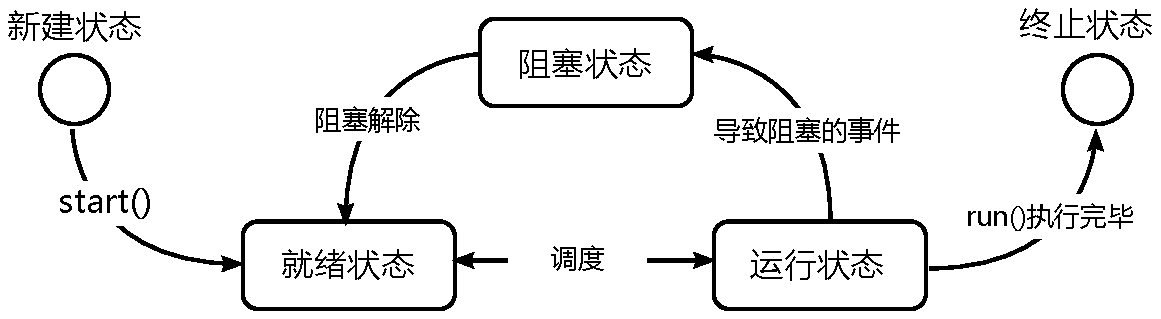
\includegraphics[width=0.95\textwidth]{images/Java-thread-programming/fig-thread-lifecycle.pdf}
\caption{Java线程生命周期状态}
\label{fig:thread-lifecycle}
\end{figure}

\subsection{线程优先级}

线程的优先级用数字来表示,范围从1到10。主线程的缺省优先级是5,子线程的
优先级默认与其父线程相同。可以使用Thread类的下述方法获得和设置线程的优
先级。

\begin{itemize}
\item 获取当前线程优先级
  \begin{javaCode}
    public final int getPriority();
  \end{javaCode}
\item 设定当前线程优先级
  \begin{javaCode}
    public final void setPriority(int newPriority);
  \end{javaCode}
\end{itemize}

相关静态整型常量如下:

\begin{javaCode}
Thread.MIN_PRIORITY = 1
Thread.MAX_PRIORITY = 10
Thread.NORM_PRIORITY = 5
\end{javaCode}

\subsection{线程串行化}

在多线程程序中,如果在一个线程运行的过程中要用到另一个线程的运行结果,
则可进行线程的串型化处理。

Thread类提供的线程串行化相关方法包括:

\begin{javaCode}
public final void join();
public final void join(long millis);
public final void join(long millis, int nanos);
\end{javaCode}

以下给出实现线程串行化的代码示例:

\samplecode{TestJoin.java}

\begin{javaCode}
public class TestJoin {
  public static void main(String[] args) {
    MyRunner r = new MyRunner();
    Thread t = new Thread(r);
    t.start();
    try {
      t.join();
    } catch(InterruptedException e) {
      e.printStackTrace();
    }
    for(int i = 0; i < 50; i++) {
      System.out.println("主线程:" + i);
    }
  }
}

class MyRunner implements Runable {
  public void run() {
    for(int i = 0; i < 50; i++) {
      System.out.println("子线程:" + i);
  }
}
\end{javaCode}

\descript{说明}

上述程序中,主线程在执行过程中调用了线程t的join()方法,该方法导致当前线程(主线程)阻塞,直
到线程t运行终止后,主线程才会获得继续执行的机会。这相当于将线程t串行加入到主线程中。

\subsection{线程休眠}

线程休眠,即暂停执行当前运行中的线程,使之进入阻塞状态,待经过指定
的“延迟时间”后再醒来并转入到就绪状态。

Thread类提供的线程休眠相关方法包括:

\begin{javaCode}
public static void sleep(long millis);
public static void sleep(long millis, int nanos);
\end{javaCode}

以下给出使用线程休眠实现的数字计数器示例:

\samplecode{Digitaltimer.java}

\begin{javaCode}
import java.util.Calendar;
import java.util.GregorianCalendar;
import javax.swing.*;

public class DigitalClock {
  public static void main(String[] args) {
    JFrame jf = new JFrame("Clock");
    JLabel clock = new JLabel("clock");
    clock.setHorizontalAlignment(JLabel.CENTER);
    jf.add(clock, "Center");
    jf.setSize(140, 80);
    jf.setLocation(500, 300);
    jf.setDefaultCloseOperation(JFrame.EXIT_ON_CLOSE);
    jf.setVisible(true);
    Thread t = new MyThread(clock);
    t.start();
  }
}

class MyThread extends Thread {
  private JLabel clock;
  private int i;
  public MyThread(JLabel clock) {
    this.clock = clock;
    this.i = 1;
  }
  public void run() {
    while(true) {
      clock.setText(String.valueOf(i++));
      try {
        Thread.sleep(1000);
      } catch(InterruptedException e) {
        e.printStackTrace();
      }
    }
  }
}  
\end{javaCode}

\subsection{线程让步}

线程让步,让运行中的线程主动放弃当前获得的CPU处理机会,但不是使该线程阻
塞,而是使之转入就绪状态。Thread类提供的线程让步相关方法:

\begin{javaCode}
public static void yield();
\end{javaCode}

以下给出一个线程让步的示例:

\samplecode{TestYield.java}

\begin{javaCode}
import java.util.Date;

public class TestYield {
  public static void main(String[] args) {
    Thread t1 = new MyThread(false);
    Thread t2 = new MyThread(true);
    Thread t3 = new MyThread(false);
    t1.start();
    t2.start();
    t3.start();
  }
}

class MyThread extends Thread {
  private boolean flag;
  public MyThread(boolean flag) {
    this.flag = flag;
  }
  public void setFlag(boolean flag) {
    this.flag = flag;
  }
  public void run() {
    long start = new Date().getTime();
    for(int i = 0; i < 200; i++) {
      if(flag) {
        Thread.yield();
      }
      System.out.println(this.getName() + ": " + i + "\t");
    }
    long end = new Date().getTime();
    System.out.println("\n" + this.getName() + "执行时间:" + (end - start) + "ms");
  }
}
\end{javaCode}

从执行结果来看,由于设置了线程让步,第二个线程明显执行时间长。调
用yield()方法只是令当前线程主动在时间片到期前使其他线程获得运行机会。

\subsection{线程挂起与恢复}

\begin{description}
\item[线程挂起] 暂时停止当前运行中的线程,使之转入阻塞状态,并且不会自动恢复运行。
\item[线程恢复] 使得一个已挂起的线程恢复运行。
\end{description}

Thread类提供的线程挂起与恢复的相关方法:

\begin{javaCode}
public final void suspend();
public final void resume();
\end{javaCode}

suspend()和resume()方法已经不提倡使用,原因是suspend()方法挂起线程时并不释放其锁定的资
源,这可能会影响到其他线程的执行,且容易导致线程死锁。

\subsection{线程等待与通知}

将运行中的线程转为阻塞状态的另外一种途径是:调用该线程中被锁定资源
(Java对象)的wait()方法,该方法在Object类中定义,其功能是让当前线程等
待,直到有其他线程调用了同一个对象的notify()或notifyAll()方法通知其结束
等待,或是经历了约定的等待时间后,等待线程才会醒来,重新进入可执行状
态。
 
线程等待与线程挂起比较:

\begin{itemize}
\item 线程挂起时不会释放所占用的资源;
\item 线程等待时则会释放资源,以使其他线程获得运行机会。
\end{itemize}

\section{线程的同步}

\subsection{临界资源问题}

两个线程A和B在同时操纵Stack类的同一个实例(栈),A向栈里push一个数据,B要从堆栈中pop一个数据。

\tta{代码}

\begin{javaCode}
public class Stack {
  int idx = 0;
  char[ ] data = new char[6];
  
  public void push(char c) {
    data[idx] = c;
    idx++;
  }
  public char pop() {
    idx--;
    return data[idx];
  }
}
\end{javaCode}

\tta{问题分析}

\begin{enumerate}
\item 操作之前,假设data = |a|b| | | | |,idx = 2;
\item 线程A执行push中的第一个语句,将c推入堆栈; data = |a|b|c| | | |,idx = 2;
\item 线程A还未执行idx++语句,A的执行被线程B中断,B执行pop方法,data = |a|b|c| | | | idx = 1;
\item 线程A继续执行push的第二个语句: data = |a|b|c| | | |, idx = 2;
\item 最后的结果相当于c没有入栈,产生这种问题的原因在于对共享数据访问的操作的不完整性。
\end{enumerate}


\subsection{什么是临界资源}

在并发程序设计中,对多线程共享的资源或数据称为{\bf\Red 临界资源}(或同
步资源),而把每个线程中访问临界资源的那一段代码称为{\bf\Blue 临界代
  码}(或临界区)。

\begin{itemize}
\item 在一个时刻只能被一个线程访问的资源就是临界资源。
\item 访问临界资源的那段代码就是临界区,{\kai\Red 临界区必须互斥地使用}。
\end{itemize}

\subsection{互斥锁}

\begin{itemize}
\item Java引入对象{\Red\hei 互斥锁}机制来实现线程的互斥操作,保证共享
  数据操作的完整性。
\item Java中每个对象都有一个互斥锁与之相连,用来保证在任一时刻,只能
  有一个线程访问该对象。
\item 多线程对临界资源的并发访问是通过竞争互斥锁实现的。
\end{itemize}

\subsection{synchronized的用法}

为了保证互斥,Java语言使用{\bf\Red synchronized}关键字标识同步的{\hei\Blue 资源},包括:

\begin{itemize}
\item 对象
  \begin{javaCode}
    synchronized(对象) {
      临界代码段
    }
  \end{javaCode}
\item 方法
  \begin{javaCode}
    public synchronized 返回值类型 方法名 {
      方法体
    }
  \end{javaCode}

  等效方式:
  
  \begin{javaCode}
    public 返回值类型 方法名 {
      synchronized(this) {
        方法体
      }
    }
  \end{javaCode}
\item 语句块(一段代码),用法同方法的等效方式
\end{itemize}

\subsection{synchronized的用法示例}

\tta{用于方法声明中,标明整个方法为同步方法}

\begin{javaCode}
  public synchronized void push(char c) {
    data[idx] = c;
    idx++;
  }
\end{javaCode}

\tta{用于修饰语句块,标明整个语句块为同步块}

\begin{javaCode}
  // Other code
  public char pop() {
    synchronized(this) {
      idx--;
      return data[idx];
    }
    // Other code
  }
\end{javaCode}

\subsection{synchronized的功能}

\begin{itemize}\kai
\item 首先判断对象或者方法的{\bf\Red 互斥锁}是或否存在,若存在就获得互斥锁,然后执行紧随其后的临界代码段或方法体;
\item 如果对象或方法的互斥锁不在(已经被其他线程拿走),就进入线程{\bf\Blue 等待状态},直到获得互斥锁。
\end{itemize}

\codeset{sample.thread.syn.WithdrawMoneyFromBankSample.java}


\subsection{线程死锁}

并发运行的多个线程间彼此等待、都无法运行的状态称为{\hei\Blue 线程死锁}。

{\kai\Red 为避免死锁,在线程进入阻塞状态时应尽量释放其锁定的资源,以为其他的线程提供运行的机会。}

\tta{相关方法}

\begin{itemize}
\item public final void wait()
\item public final void notify()
\item public final void notifyAll()
\end{itemize}

\subsection{线程间通信}

通过线程间的{\Red\hei 对话}来解决线程间的同步问题。

\tta{线程间通信的有效手段}

\ttc{wait()} {\small\kai 如果一个正在执行同步代码(synchronized)的线
  程A执行了wait()调用(在对象x上),该线程暂停执行而进入对象x的等待队
  列,并释放已获得的对象x的互斥锁。线程A要一直等到其他线程在对象x上调
  用notify()或notifyAll()方法,才能重新获得对象x的互斥锁后继续执行
  (从wait()语句后继续执行)。}

\ttc{notify()} {\small\kai 唤醒正在等待该对象互斥锁的第一个线程。}

\ttc{notifyAll()} {\small\kai 唤醒正在等待该对象互斥锁的所有线程,具有最高优先级的线程首先被唤醒并执行。}
  

\subsection{Object.wait()和notify()}

\begin{itemize}
\item wait()和notify()只能在同步代码块中调用。
\item wait()在放弃CPU资源的同时交出了对资源的控制权。
\end{itemize}


\subsection{Thread.sleep()与Object.wait()、notify()的区别}
  
\begin{itemize}
\item 所属对象不同。sleep()是Thread类的方法,
  而wait(),notify(),notifyAll()是Object类中定义的方法,都会影响线程
  的执行行为。
\item 锁行为不同。Thread.sleep()不会导致锁行为的改变,如果当前
  线程是拥有锁的,那么Thread.sleep()不会让线程释放锁。可以简单认为和
  锁相关的方法都定义在Object类中,因此调用Thread.sleep()不会影响锁
  的相关行为。
\item 线程恢复方式不同。Thread.sleep和Object.wait都会暂停当前的
  线程,即表示它暂时不再需要CPU的执行时间。区别是调用wait后,需要别的
  线程执行notify/notifyAll才能够重新获得CPU执行时间。
\end{itemize}

\subsection{生产者—消费者问题}

生产者消费者模型(如图\ref{fig:producer-and-consumer})就是在一个系统中
存在{\hei\Red 生产者}和{\hei\Red 消费者}两种角色,他们之间通
过{\hei\Blue 内存缓冲区}进行通信,生产者生产消费者需要的资料,消费者把
资料做成产品。
  
\tta{生产者消费者问题是线程模型中的经典问题}

\begin{itemize}
\item 生产者和消费者在同一时间段内共用同一存储空间,生产者向空间里生
  产数据,而消费者取走数据。
\item 阻塞队列就相当于一个缓冲区,平衡了生产者和消费者的处理能力。这
  个阻塞队列就是用来给生产者和消费者解耦的。
\end{itemize}

\begin{figure}[htb]
\centering
\framebox{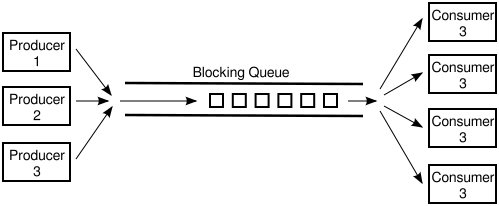
\includegraphics[width=0.8\textwidth]{images/Java-thread-programming/producer-and-consumer.png}}
\caption{生产者消费者问题}
\label{fig:producer-and-consumer}
\end{figure}

\codeset{sample.thread.syn.ProducerAndConsumer.java}

\section{课后习题}

\tta{简答题}

\begin{enumerate}
\item 简述线程的基本概念。程序、进程、线程的关系是什么?
\item 线程的生命周期包括哪些基本状态?这些状态的关系如何?状态间的切
  换控制如何进行?({\kai\Blue 可以通过思维导图、文字描述等方式梳理线
    程状态与控制转换方法之间的关系})
\end{enumerate}

\tta{小编程}

\begin{enumerate}
\item 编程实践生产者—消费者模式,并在理解的基础上对代码给出比较完整的注释。
\end{enumerate}